\documentclass{article}%
\usepackage[T1]{fontenc}%
\usepackage[utf8]{inputenc}%
\usepackage{lmodern}%
\usepackage{textcomp}%
\usepackage{lastpage}%
\usepackage[head=40pt,margin=0.5in,bottom=0.6in]{geometry}%
\usepackage{graphicx}%
%
\title{\textbf{Habitantes de Barquisimeto protestan por deficiencia de servicios públicos}}%
\author{El Nacional Web}%
\date{19/11/2018}%
%
\begin{document}%
\normalsize%
\maketitle%
\textbf{URL: }%
http://www.el{-}nacional.com/noticias/protestas/habitantes{-}barquisimeto{-}protestan{-}por{-}deficiencia{-}servicios{-}publicos\_260283\newline%
%
\textbf{Periodico: }%
EN, %
ID: %
260283, %
Seccion: %
Protestas\newline%
%
\textbf{Palabras Claves: }%
Lara, Protestas, Denuncia\newline%
%
\textbf{Derecho: }%
2.8%
, Otros Derechos: %
NO\_TIENE%
, Sub Derechos: %
2.8.1%
\newline%
%
\textbf{EP: }%
SI\newline%
\newline%
%
\textbf{\textit{Los manifestantes bloquearon diversas vías de accesos como medida de protesta por la falta de gas doméstico}}%
\newline%
\newline%
%
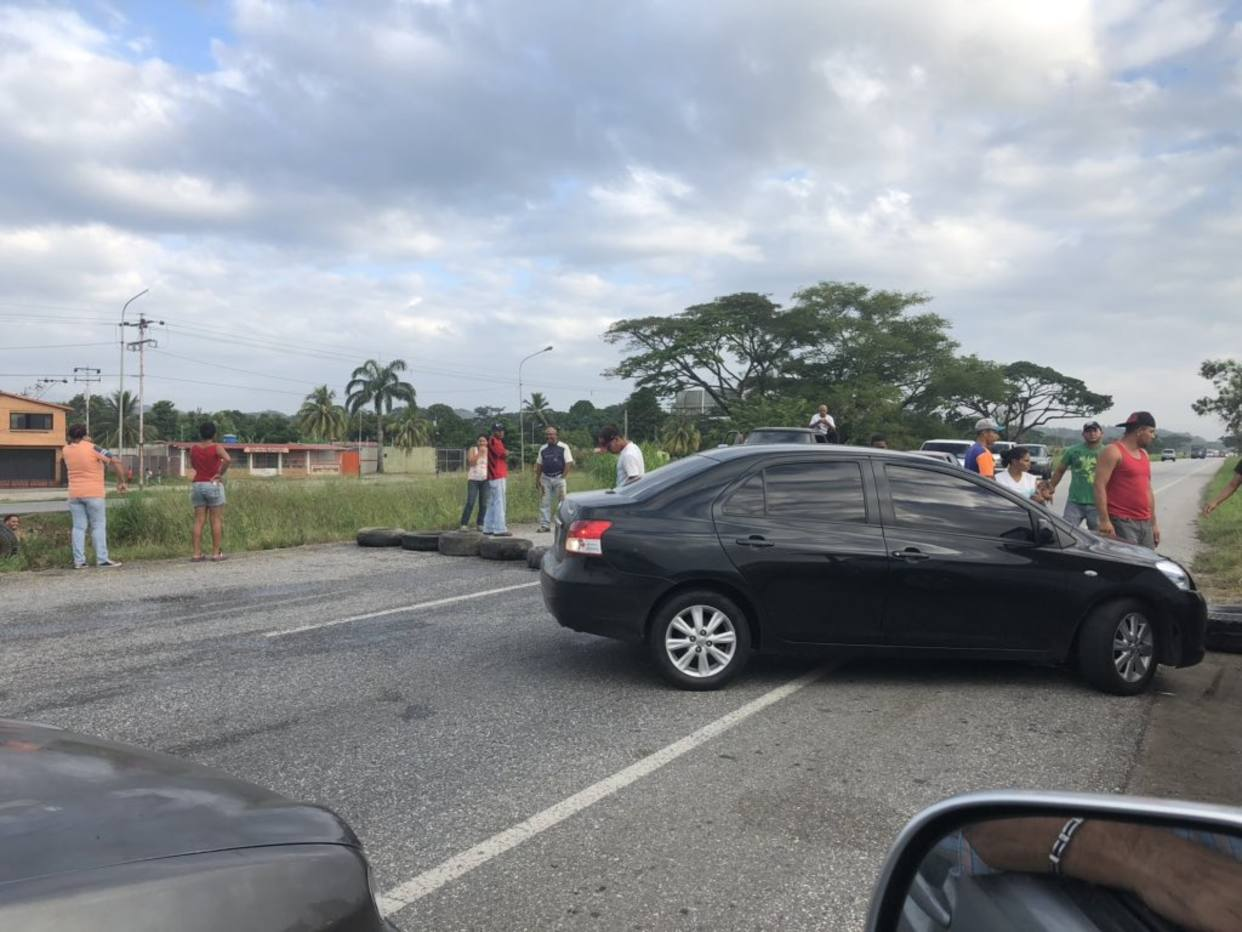
\includegraphics[width=300px]{174.jpg}%
\newline%
%
Habitantes de la ciudad de Barquisimeto, estado Lara,~ protestan este lunes debido a la deficiencia de los servicios públicos y la escasez del gas doméstico en diversas zonas de la capital.%
\newline%
%
Los manifestantes bloquearon los accesos de las vías hacia Río Claro por la falta de gas, y también en el sector El Milagro en la autopista Barquisimeto {-} Acarigua en el que efectivos de la Guardia Nacional Bolivariana (GNB) han haecho acto de presencia.%
\newline%
%
En diversas entidades del país se han registrado numerosas manifestaciones debido a la escasez del gas doméstico y la falta de respuesta por parte de las empresas que suministran el servicio básico.%
\newline%
%
\end{document}